\chapter*{L'\'Equateur, de Cuenca à Baños\markboth{L'\'Equateur, de Cuenca à Baños}{}}
\section*{22 juin 2015}
Je quitte le Pérou depuis Trujillo en bus vers Cuenca : 4h de bus jusqu'à Chiclayo, suivi d'un bus de nuit vers l'Équateur avec passage de la frontière au milieu de la nuit. Cuenca est une jolie ville située à 2500m d'altitude dans la sierra équatorienne. Le climat est frais et le temps très instable comme je vais m'en apercevoir sur la route ensuite. 
\begin{center} 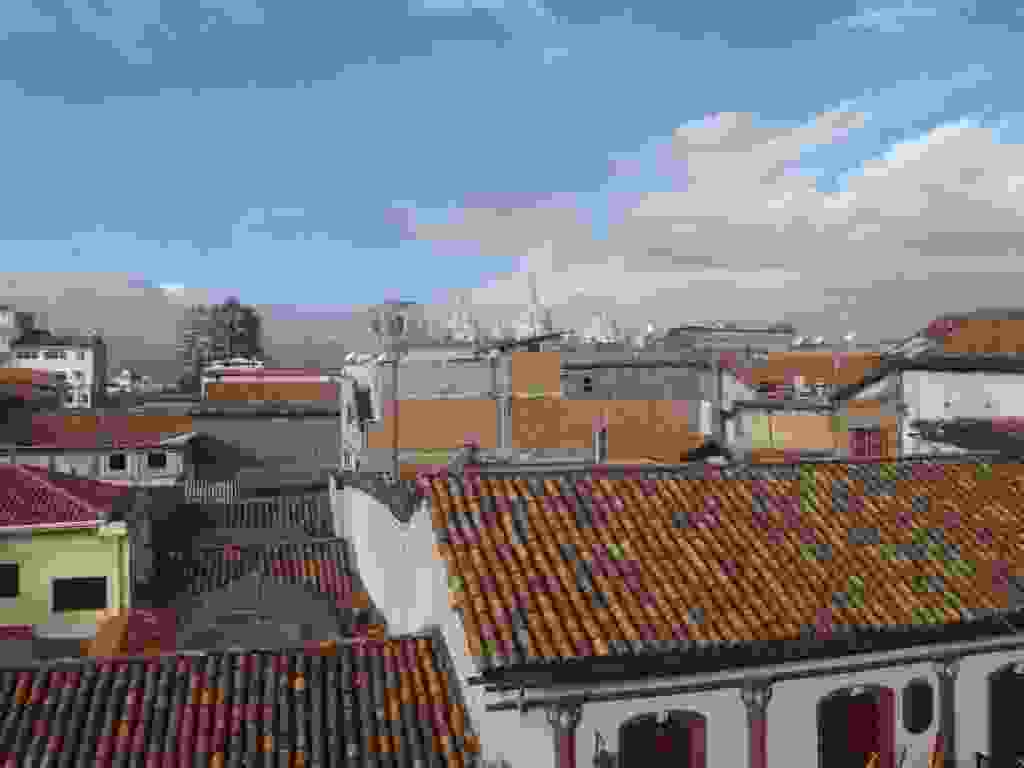
\includegraphics[width=\mywidth]{../wp-content/uploads/2015/06/P6124839-1024x768.jpg} \end{center}
\begin{center} 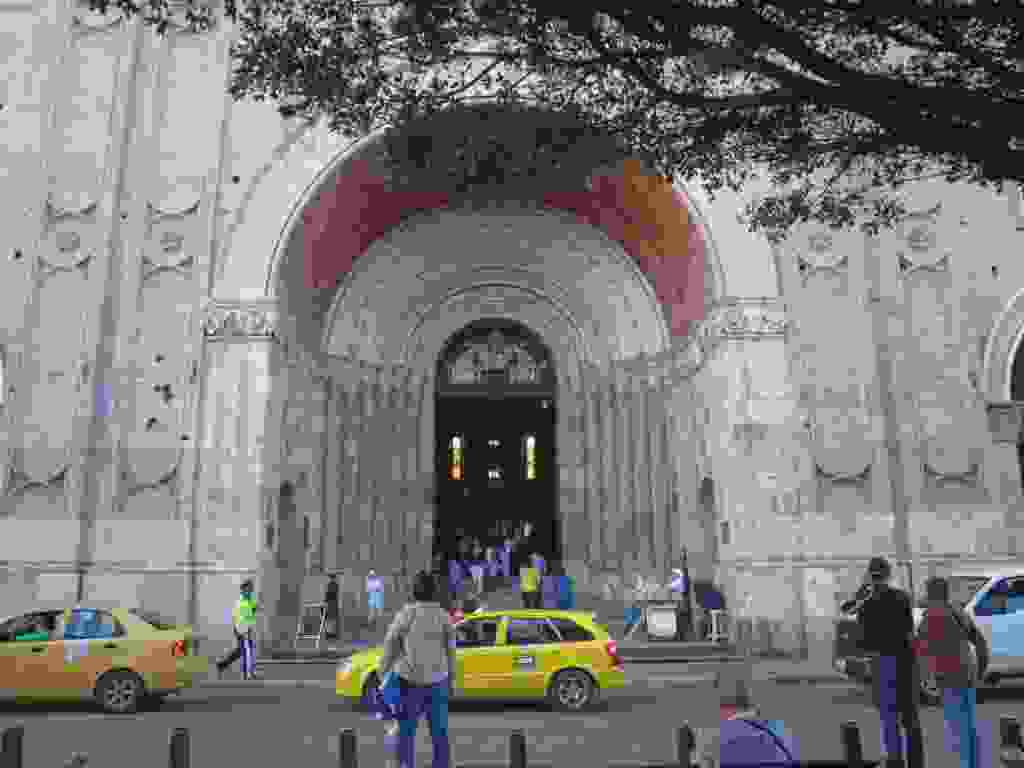
\includegraphics[width=\mywidth]{../wp-content/uploads/2015/06/P6124844-1024x768.jpg} \end{center}
\begin{center} 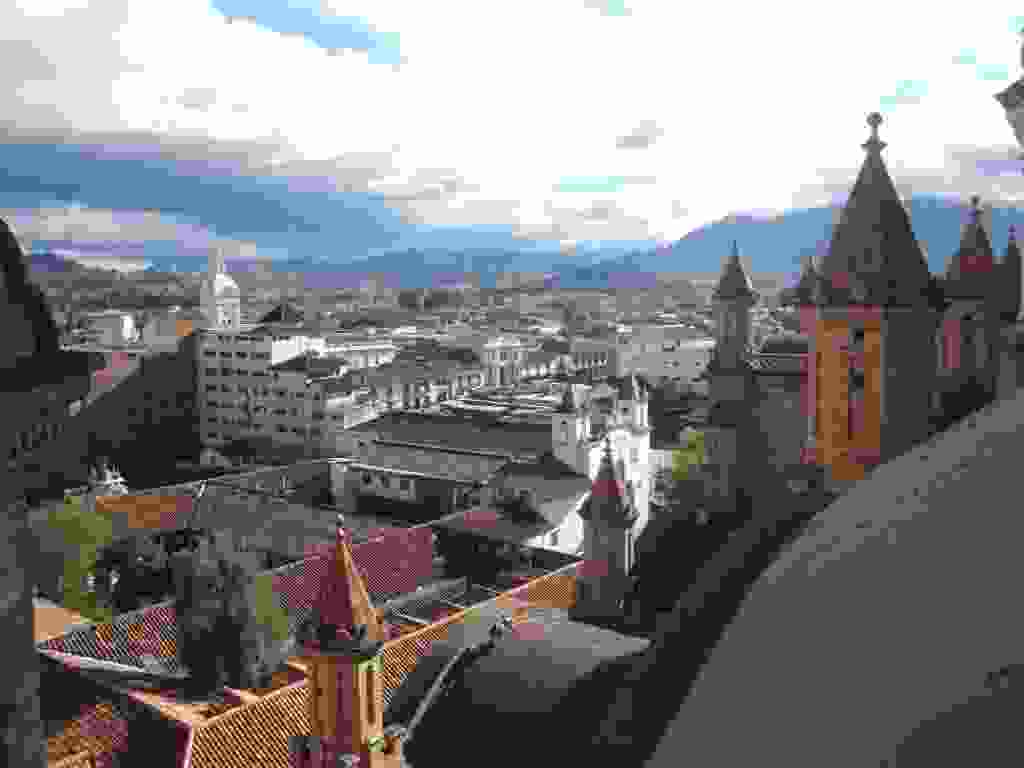
\includegraphics[width=\mywidth]{../wp-content/uploads/2015/06/P6124846-1024x768.jpg} \end{center}
\begin{center} 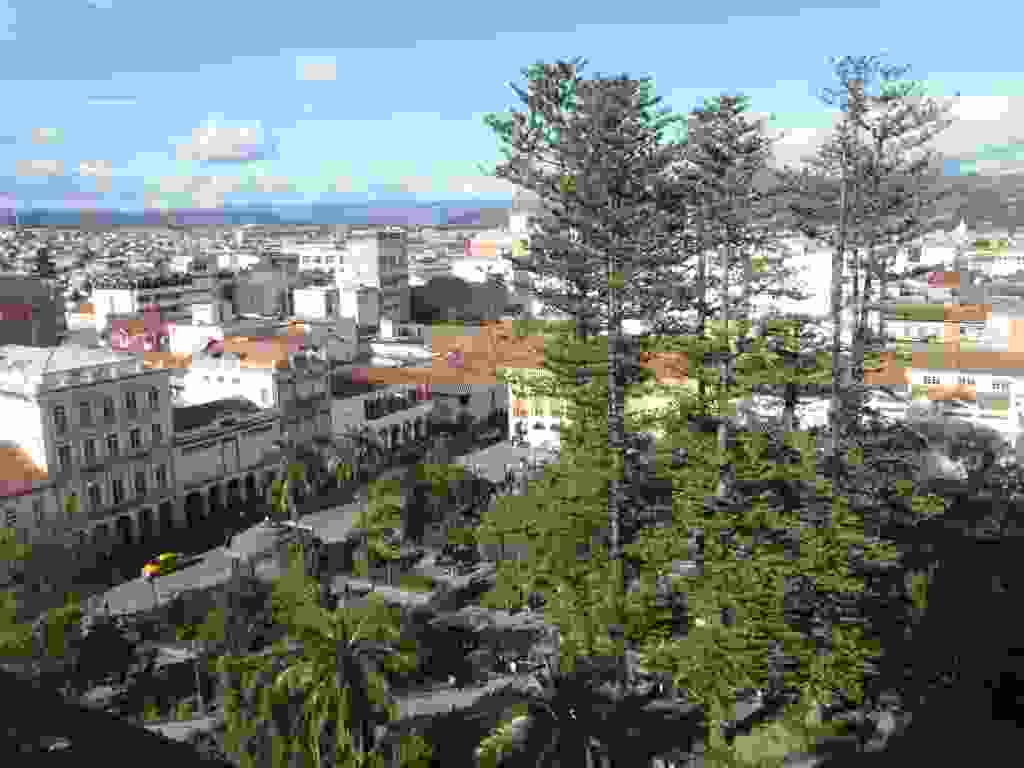
\includegraphics[width=\mywidth]{../wp-content/uploads/2015/06/P6124849-1024x768.jpg} \end{center}
\begin{center} 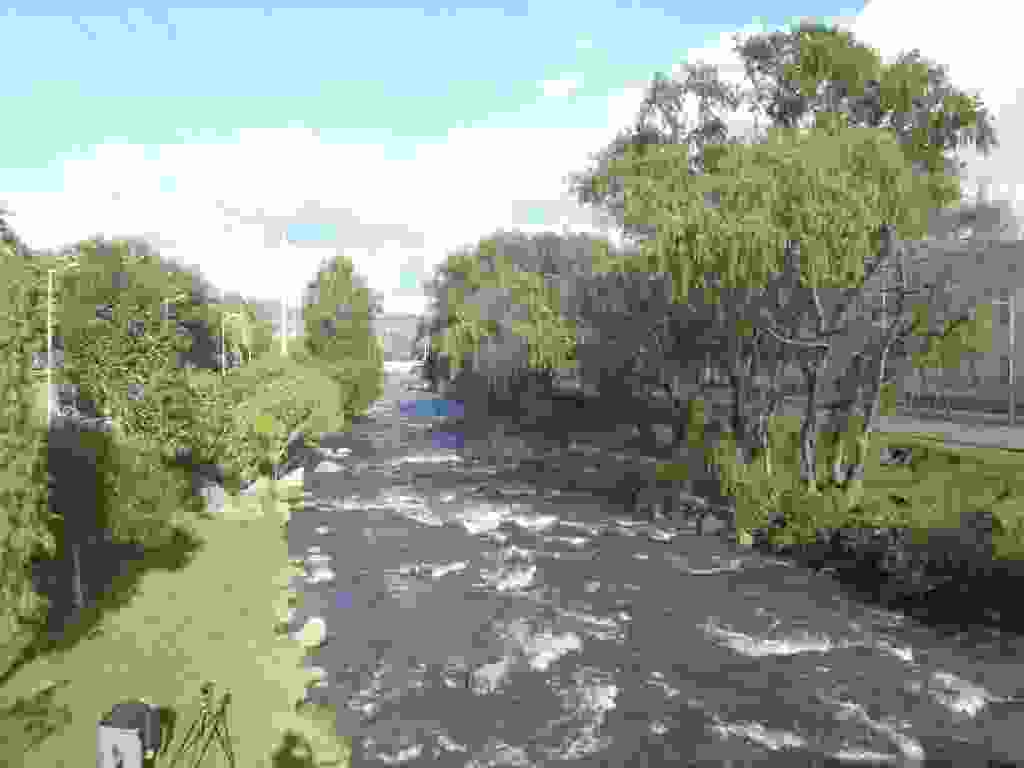
\includegraphics[width=\mywidth]{../wp-content/uploads/2015/06/P6124852-1024x768.jpg} \end{center}
\pagebreak

Encore beaucoup de fruits dans les marchés ici. 
\begin{center} 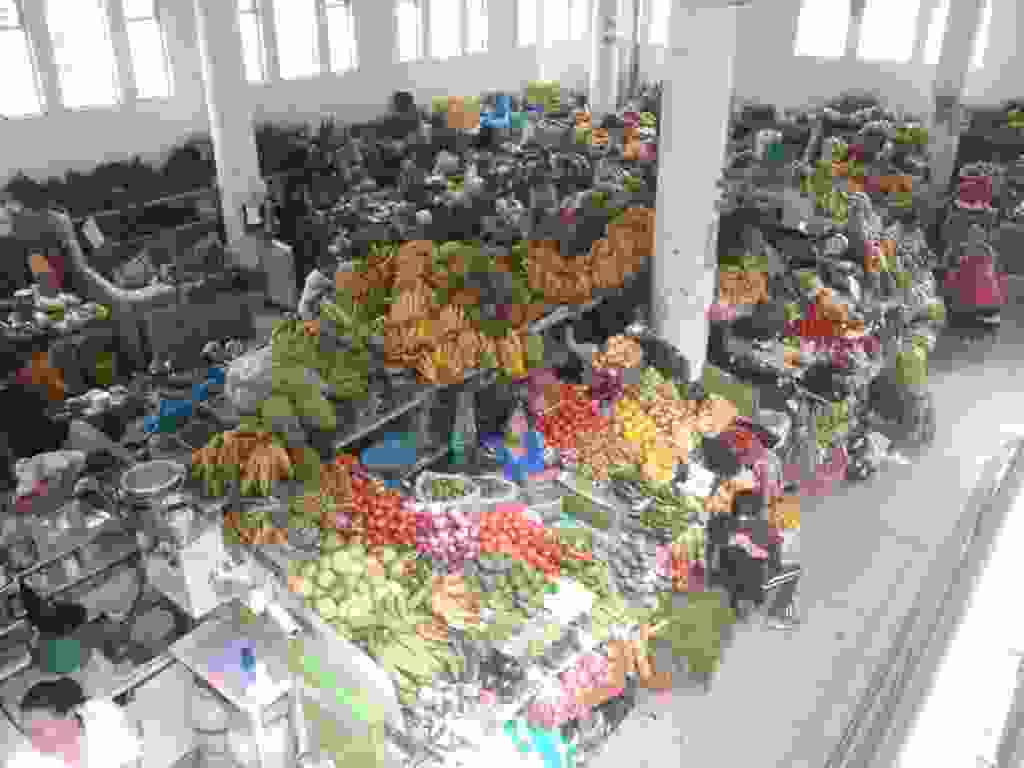
\includegraphics[width=\mywidth]{../wp-content/uploads/2015/06/P6134855-1024x768.jpg} \end{center}

Je visite le musée archéologique. 
\begin{center} 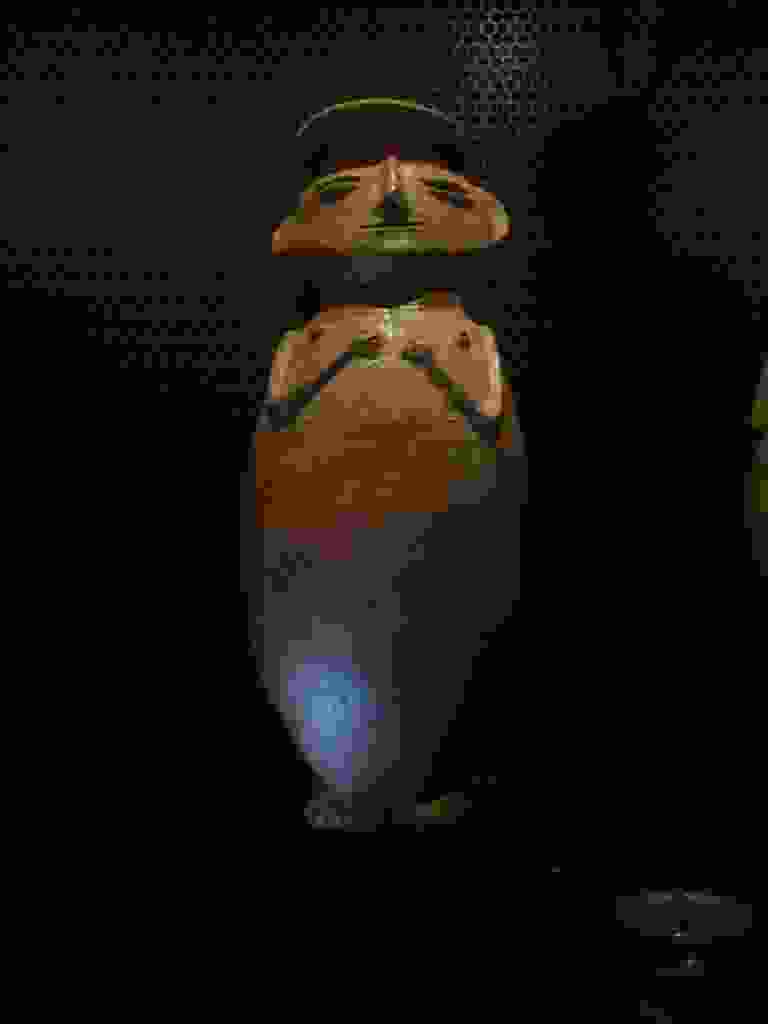
\includegraphics[height=0.82\textwidth]{../wp-content/uploads/2015/06/P6134859-768x1024.jpg} \end{center}
\pagebreak

Puis une balade au parc national Cajas près de Cuenca. 
\begin{center} 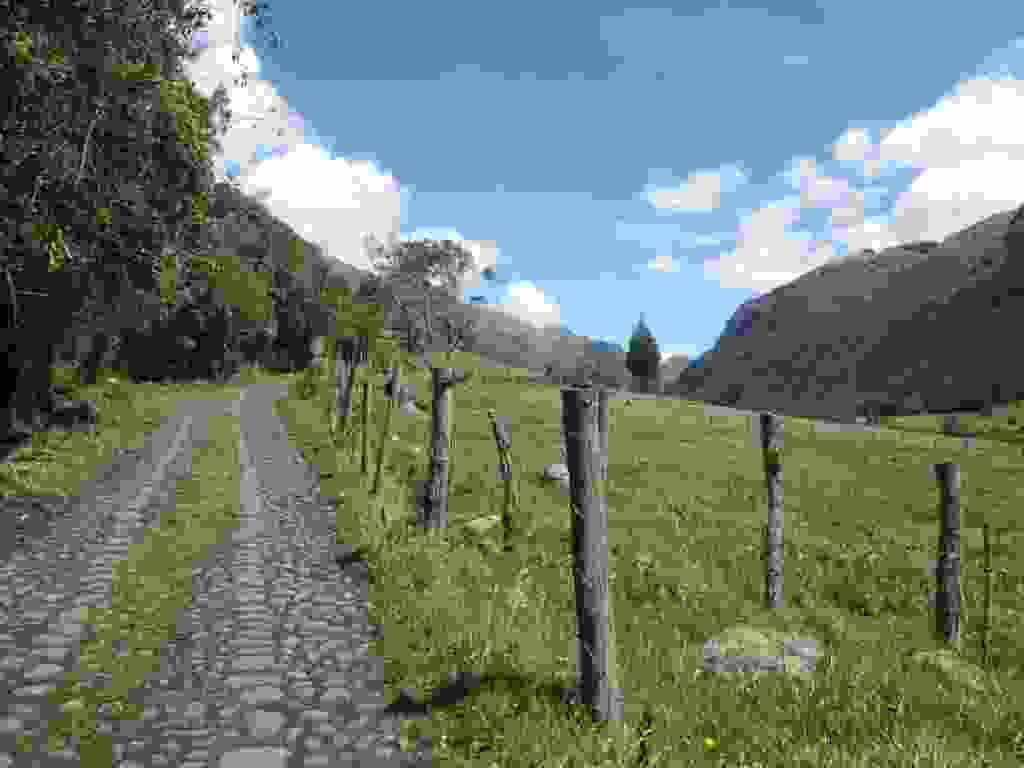
\includegraphics[width=\mywidth]{../wp-content/uploads/2015/06/P6144861-1024x768.jpg} \end{center}
\begin{center} 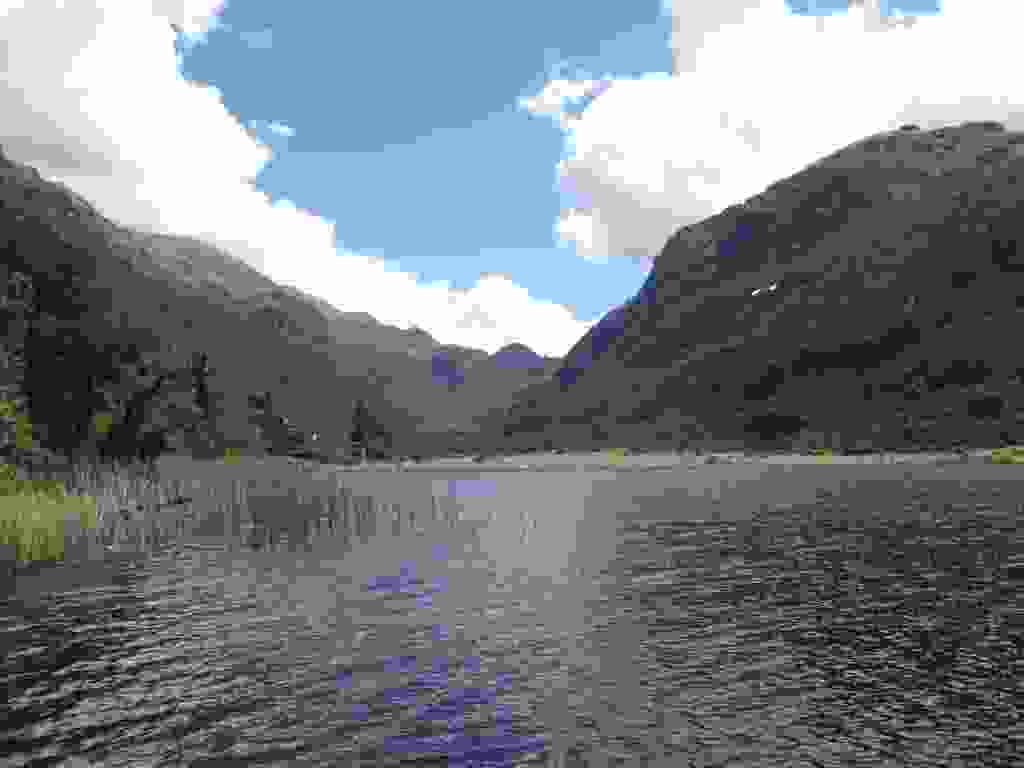
\includegraphics[width=\mywidth]{../wp-content/uploads/2015/06/P6144868-1024x768.jpg} \end{center}
\begin{center} 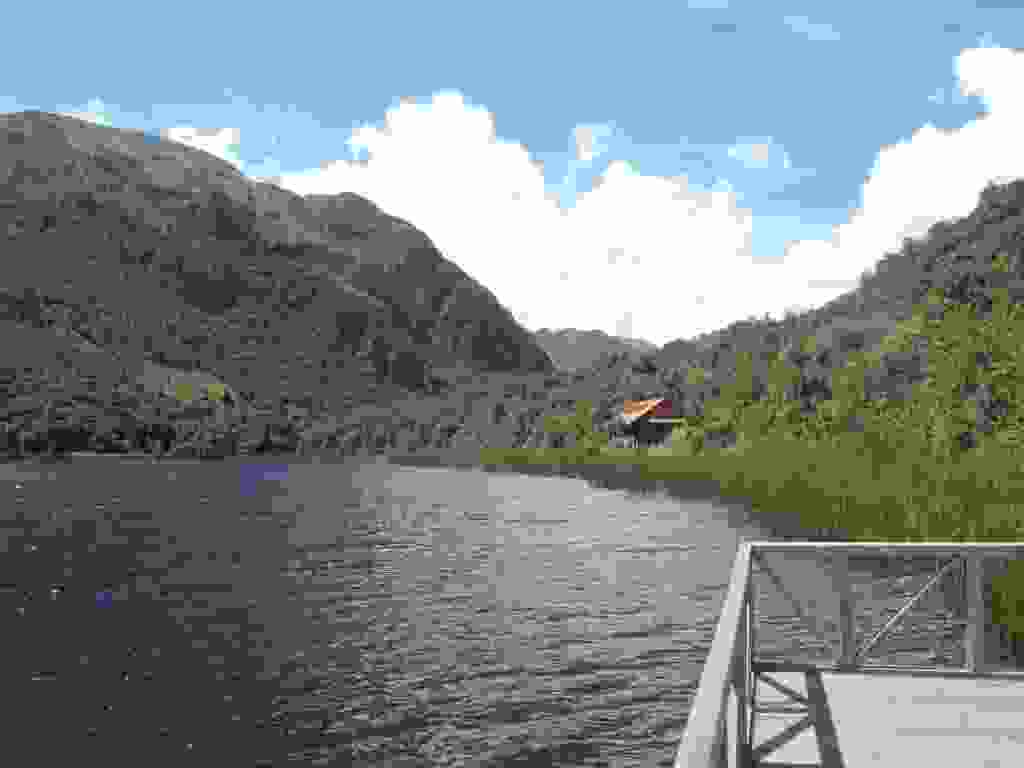
\includegraphics[width=\mywidth]{../wp-content/uploads/2015/06/P6144869-1024x768.jpg} \end{center}
\begin{center} 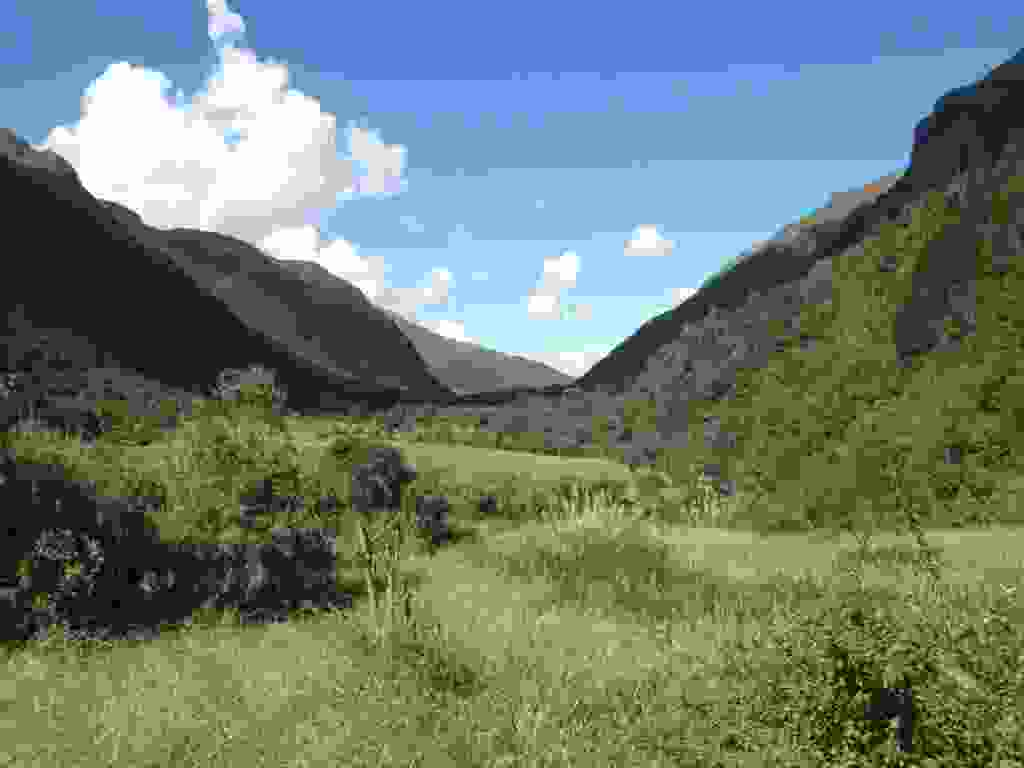
\includegraphics[width=\mywidth]{../wp-content/uploads/2015/06/P6144878-1024x768.jpg} \end{center}
\pagebreak

J'avais prévu de camper une nuit dans le parc mais l'état du chemin me fait faire demi-tour et rentrer à Cuenca. 
\begin{center} 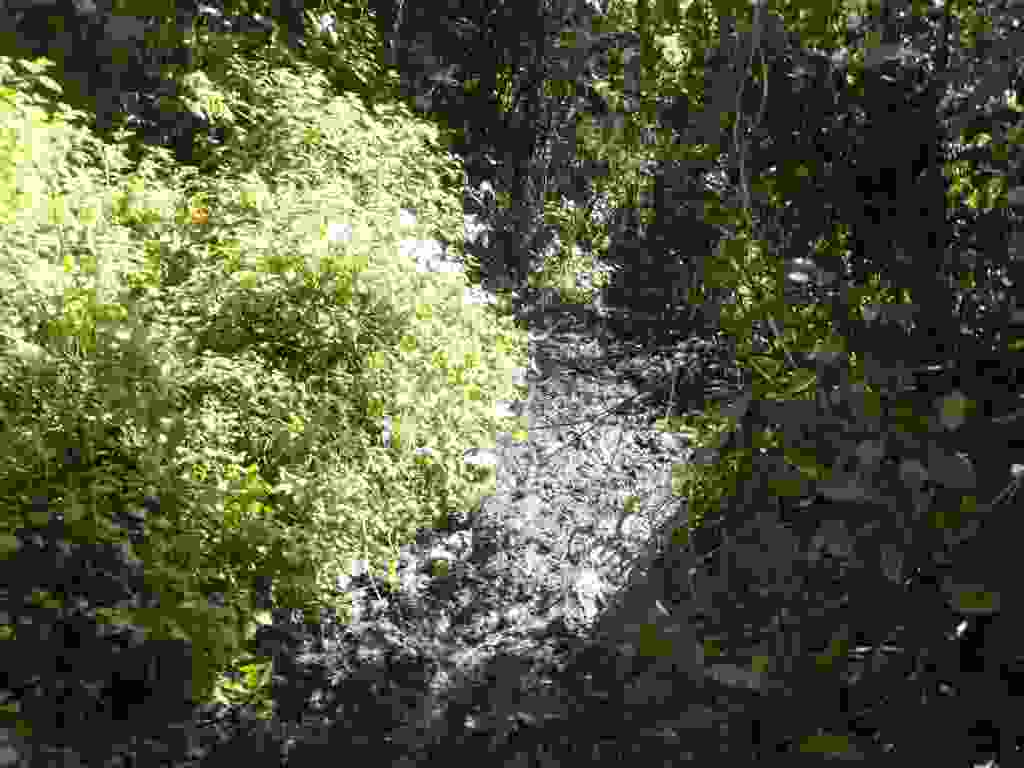
\includegraphics[width=\mywidth]{../wp-content/uploads/2015/06/P6144872-1024x768.jpg} \end{center}

Je prends ensuite la route vers le nord pour une traversée de l'Équateur par les montagnes. 
\begin{center} 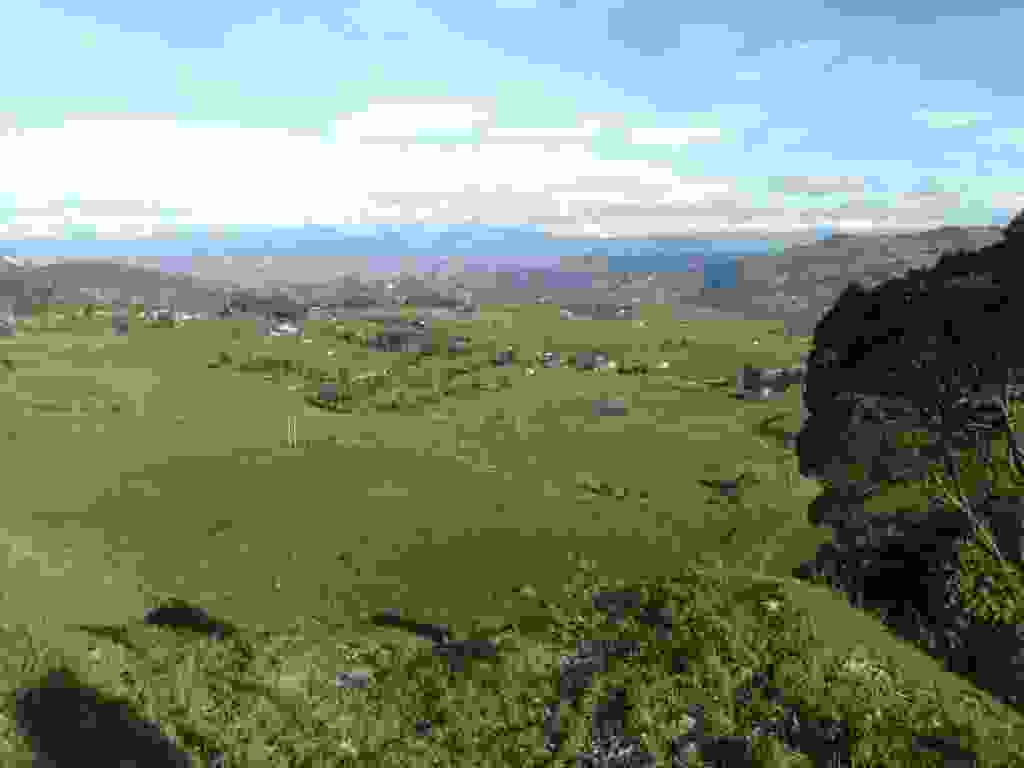
\includegraphics[width=\mywidth]{../wp-content/uploads/2015/06/P6154884-1024x768.jpg} \end{center}
\begin{center} 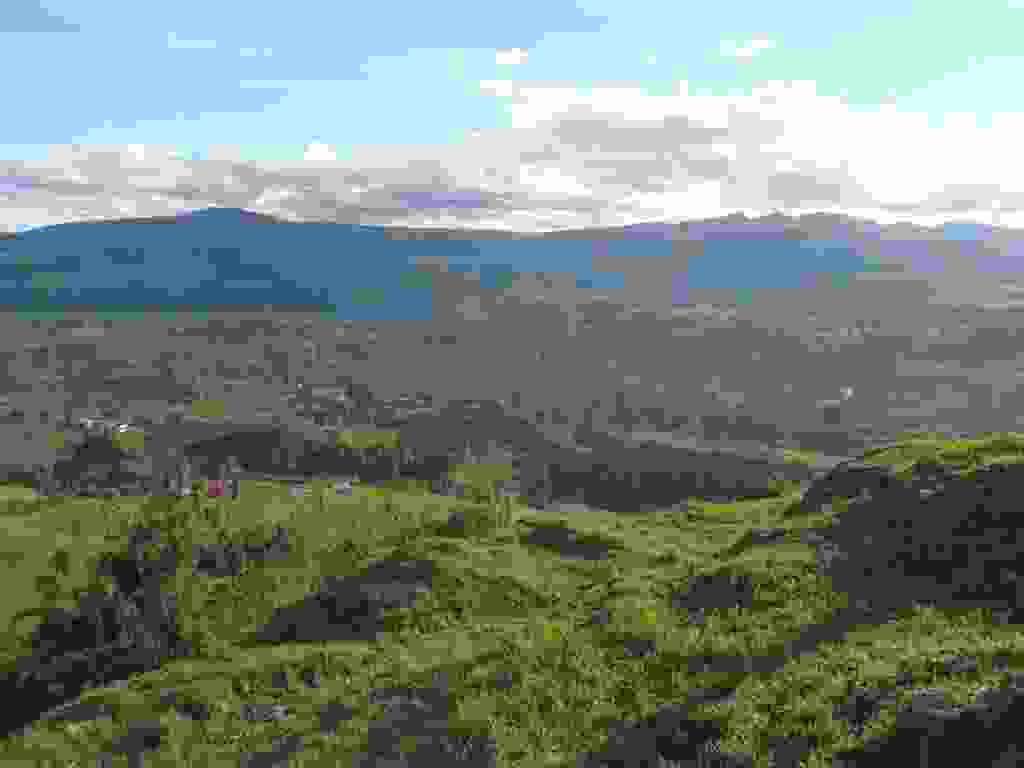
\includegraphics[width=\mywidth]{../wp-content/uploads/2015/06/P6154885-1024x768.jpg} \end{center}

La région est très agricole, je peux observer les cultures associées de maïs et haricots. 
\begin{center} 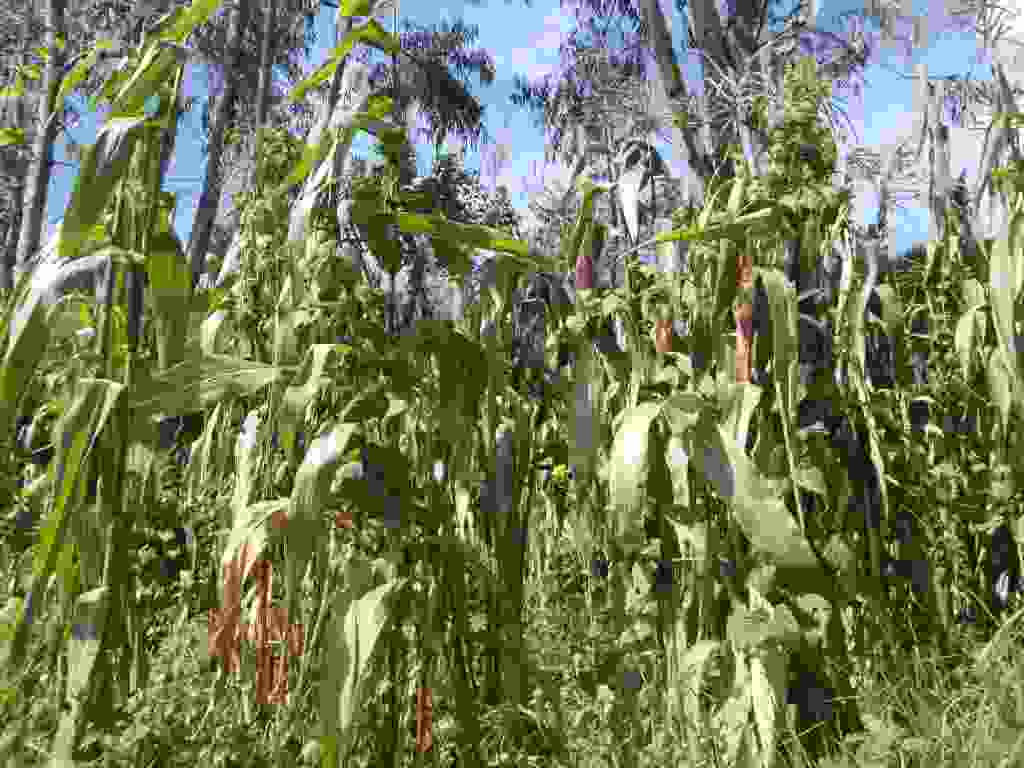
\includegraphics[width=\mywidth]{../wp-content/uploads/2015/06/P6154881-1024x768.jpg} \end{center}
\pagebreak

Beaucoup de chiens aussi, l'un d'entre eux a essayé de manger une sacoche arrière, heureusement c'est solide.

Pause dans le village d'El Tambo. 
\begin{center} 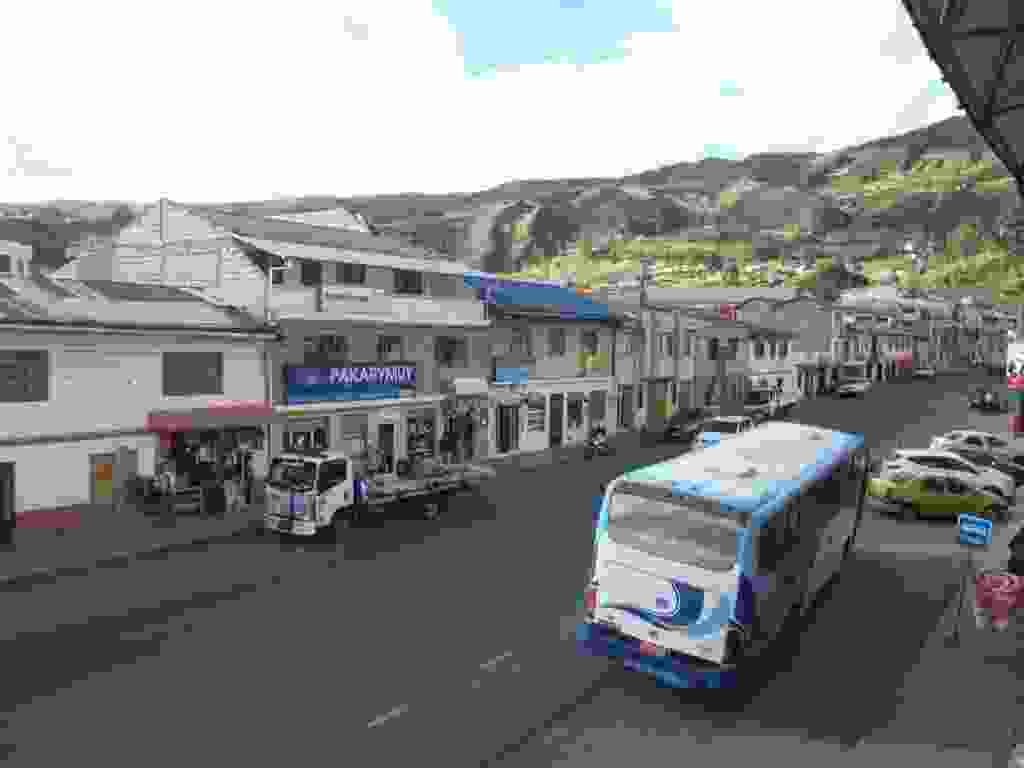
\includegraphics[width=\mywidth]{../wp-content/uploads/2015/06/P6164891-1024x768.jpg} \end{center}

La route continue avec un enchaînement de cols, ça monte bien ! 
\begin{center} 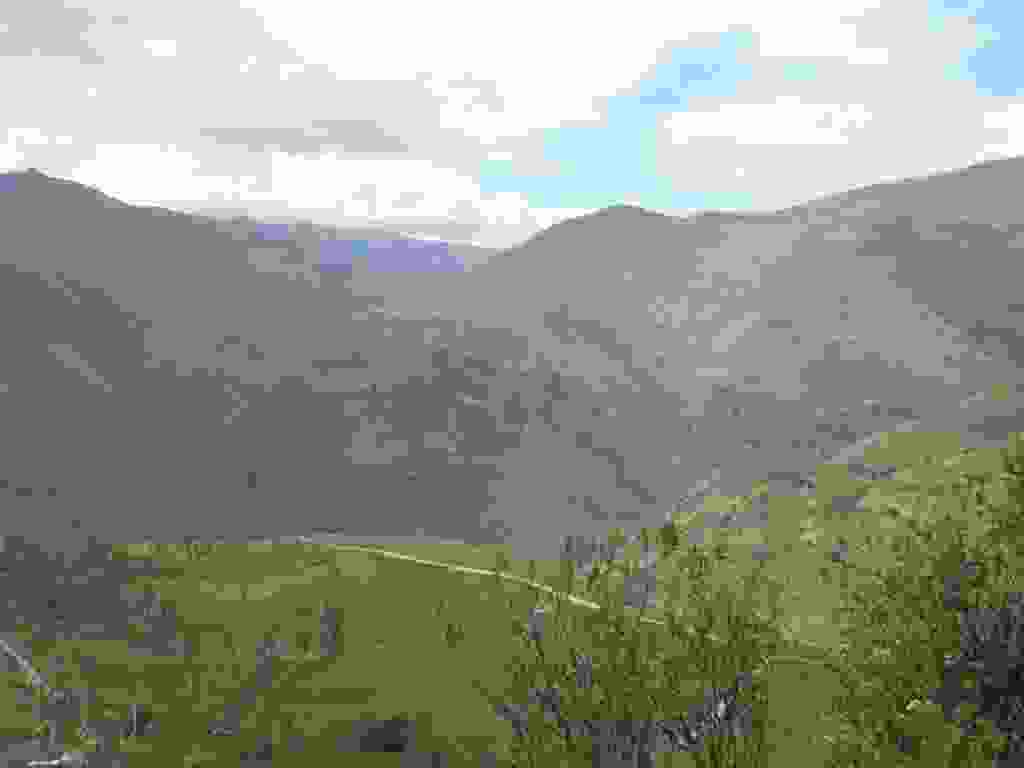
\includegraphics[width=\mywidth]{../wp-content/uploads/2015/06/P6174899-1024x768.jpg} \end{center}
\begin{center} 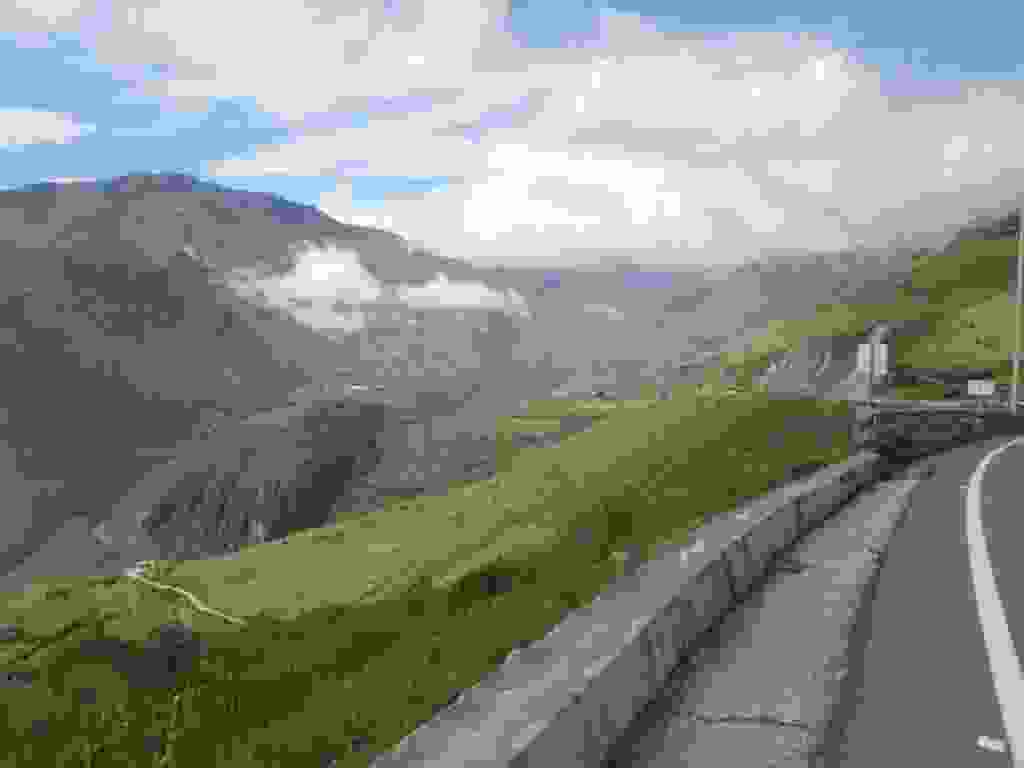
\includegraphics[width=\mywidth]{../wp-content/uploads/2015/06/P6174901-1024x768.jpg} \end{center}

Bivouac au dessus de la petite ville d'Alausi. 
\begin{center} 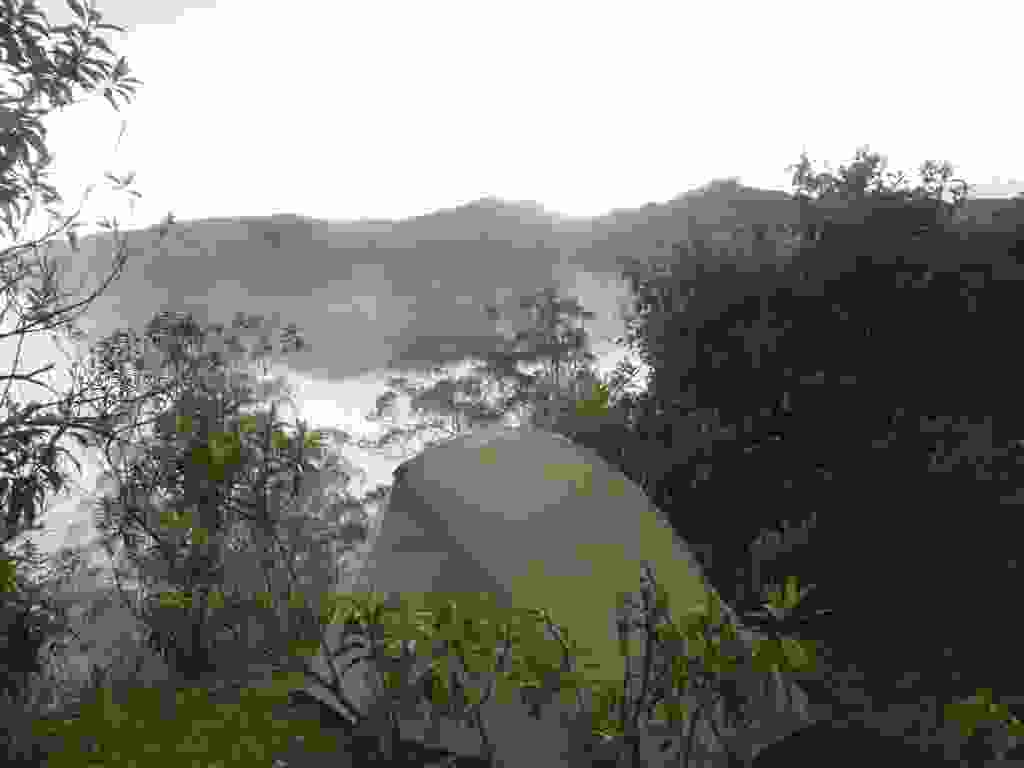
\includegraphics[width=\mywidth]{../wp-content/uploads/2015/06/P6184909-1024x768.jpg} \end{center}
\begin{center} 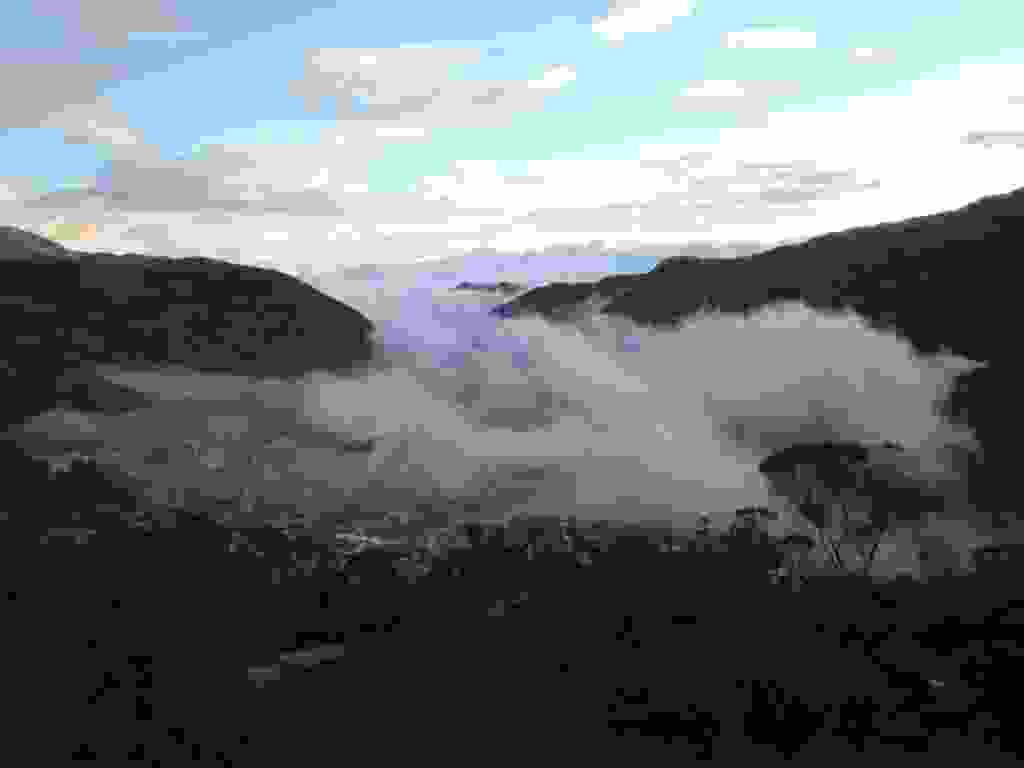
\includegraphics[width=\mywidth]{../wp-content/uploads/2015/06/P6184910-1024x768.jpg} \end{center}

Je m'arrête dans un village pour faire des courses, un jeune me demande d'essayer le vélo. J'hésite mais je le laisse faire : l'erreur, après seulement 5m il tombe et casse la béquille du vélo ! Au moins le vélo sera un peu plus léger maintenant...
Encore des kilomètres et du dénivelé avant de passer par Riobamba. 
\begin{center} 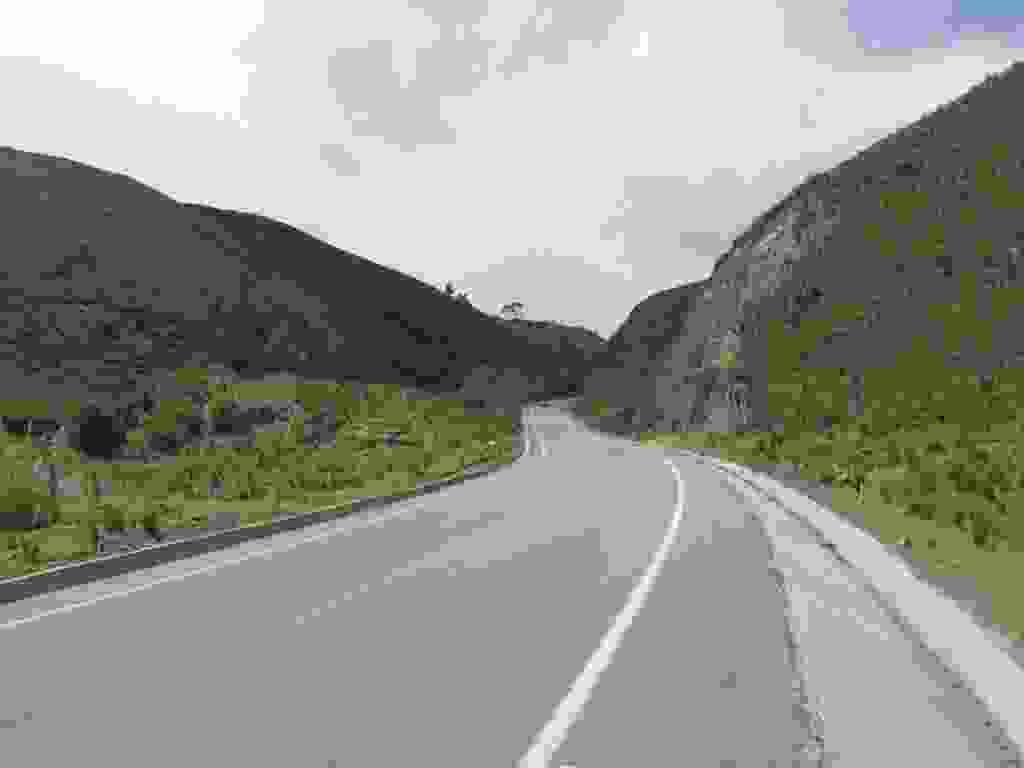
\includegraphics[width=\mywidth]{../wp-content/uploads/2015/06/P6184917-1024x768.jpg} \end{center}
\begin{center} 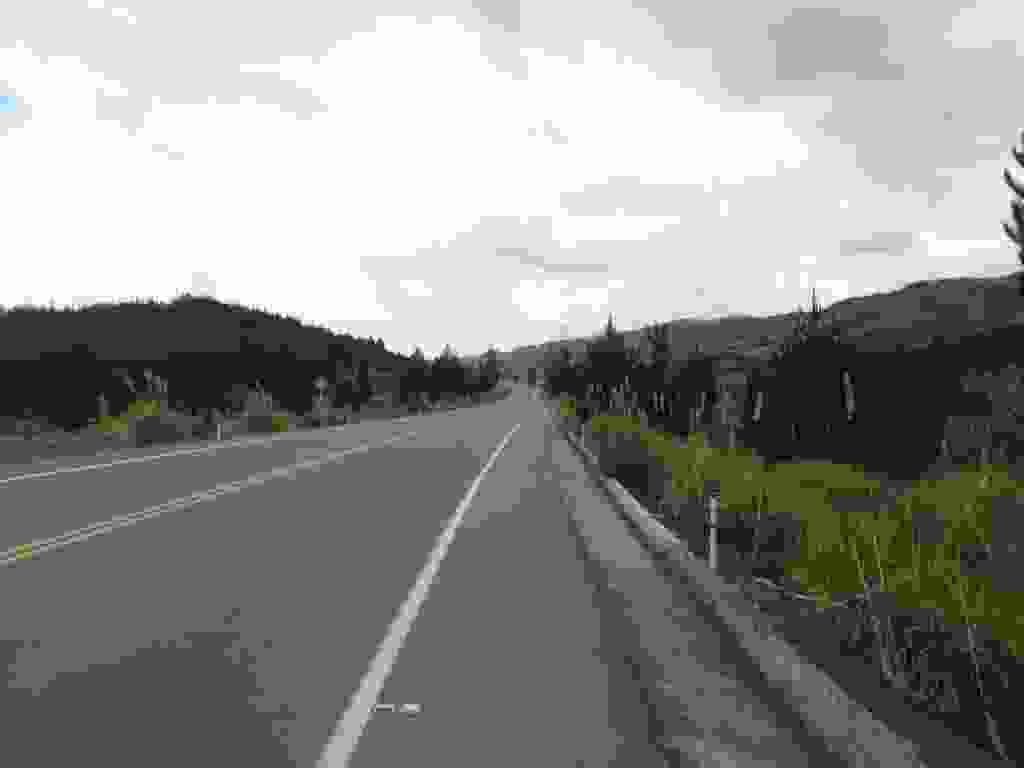
\includegraphics[width=\mywidth]{../wp-content/uploads/2015/06/P6184918-1024x768.jpg} \end{center}
\begin{center} 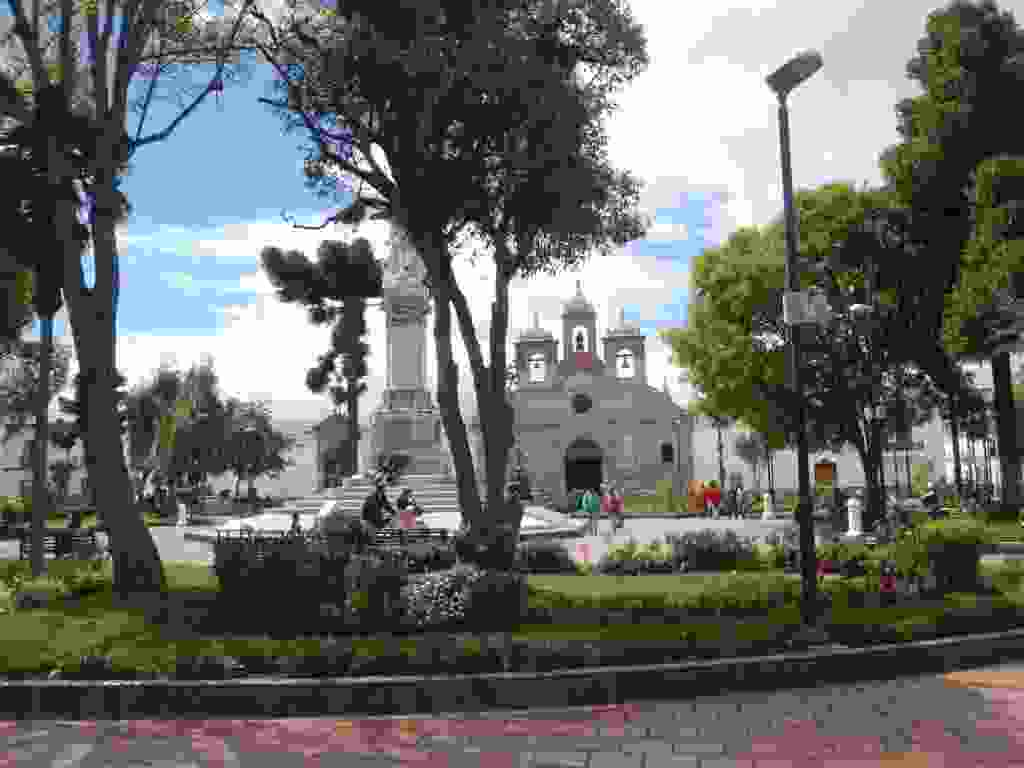
\includegraphics[width=\mywidth]{../wp-content/uploads/2015/06/P6194924-1024x768.jpg} \end{center}
\pagebreak

La dernière journée avant Baños est sous la pluie et dans le brouillard, en plus je me trompe de route et je fais un détour de 10km, en montée bien sûr ! La vue est inexistante mais heureusement des panneaux placés tous les km donnent des conseils écologiques fort utiles. 
\begin{center} 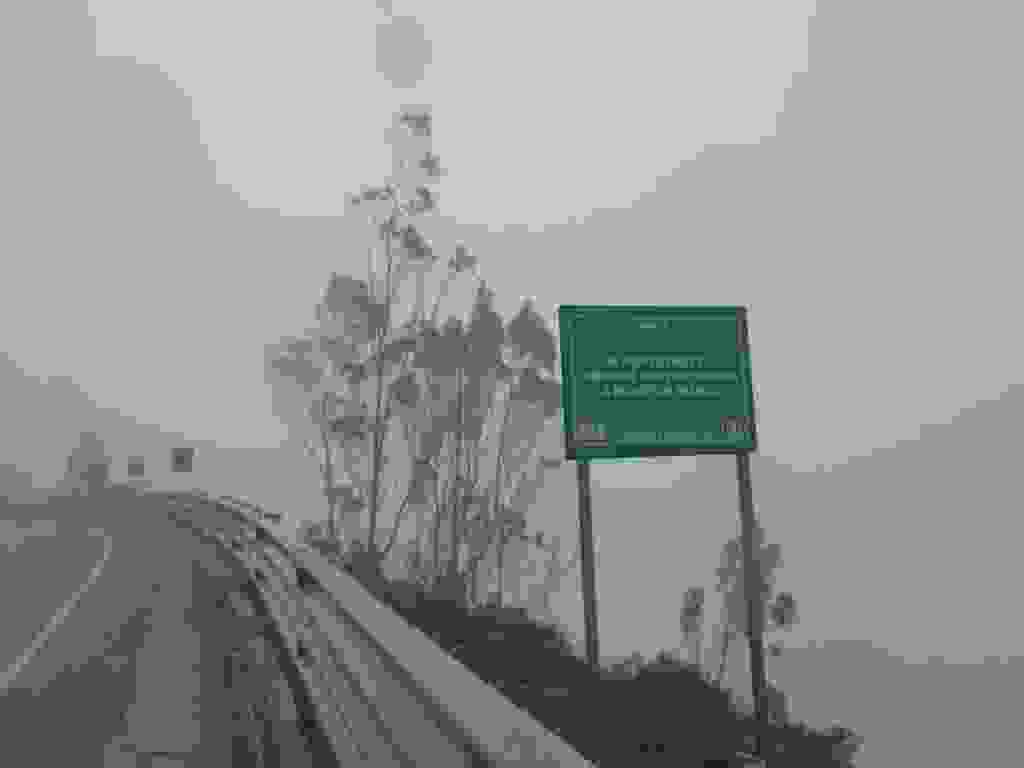
\includegraphics[width=\mywidthreduced]{../wp-content/uploads/2015/06/P6204934-1024x768.jpg} \end{center}

J'arrive enfin à Baños de Agua Santa dans les montagnes, réputée pour ses bains chauds mais surtout pour les activités sportives à proximité : rafting, canyoning, vélo, randonnées... 
\begin{center} 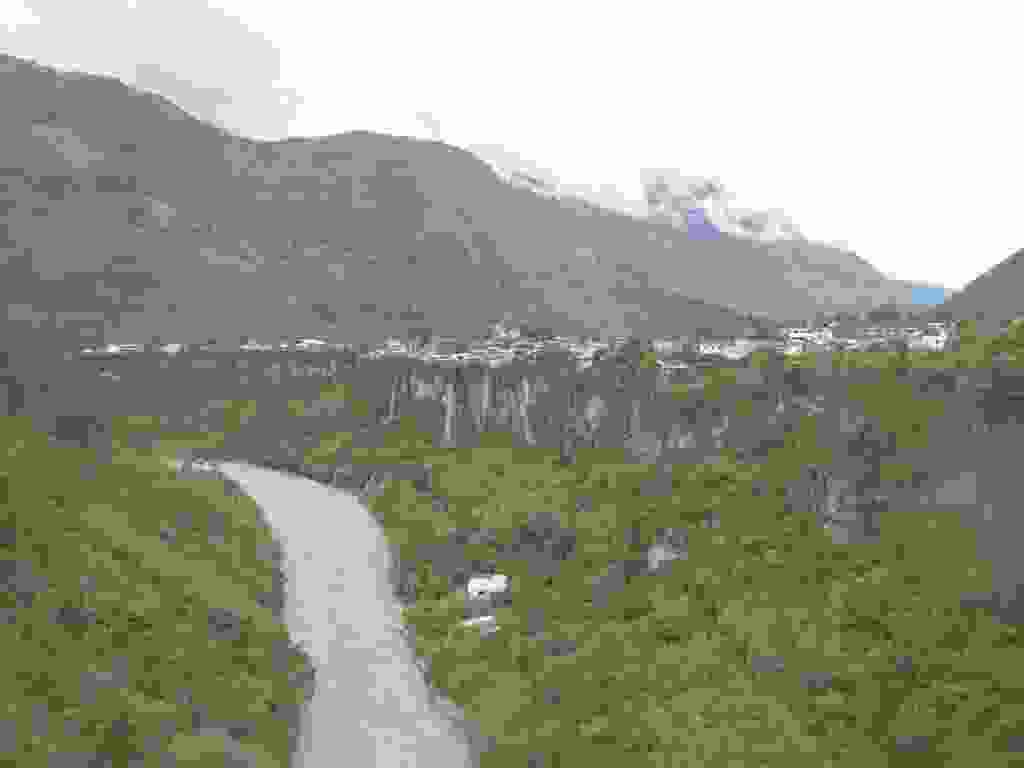
\includegraphics[width=\mywidthreduced]{../wp-content/uploads/2015/06/P6214949-1024x768.jpg} \end{center}
\begin{center} 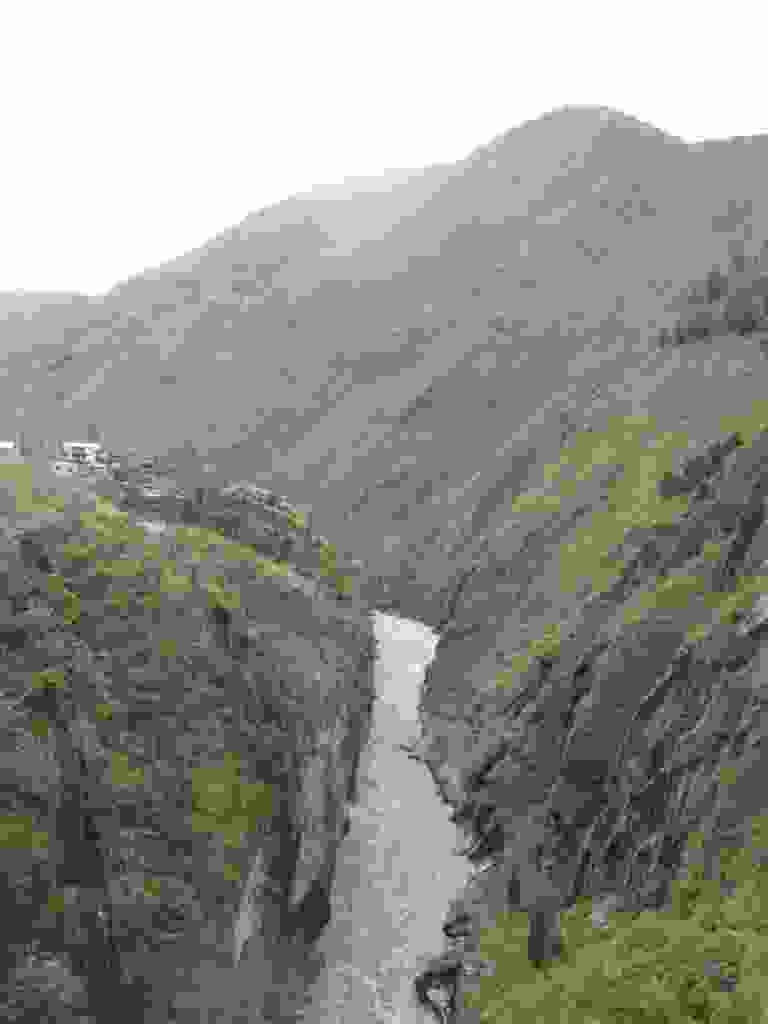
\includegraphics[height=\mywidth]{../wp-content/uploads/2015/06/P6214951-768x1024.jpg} \end{center}
\begin{center} 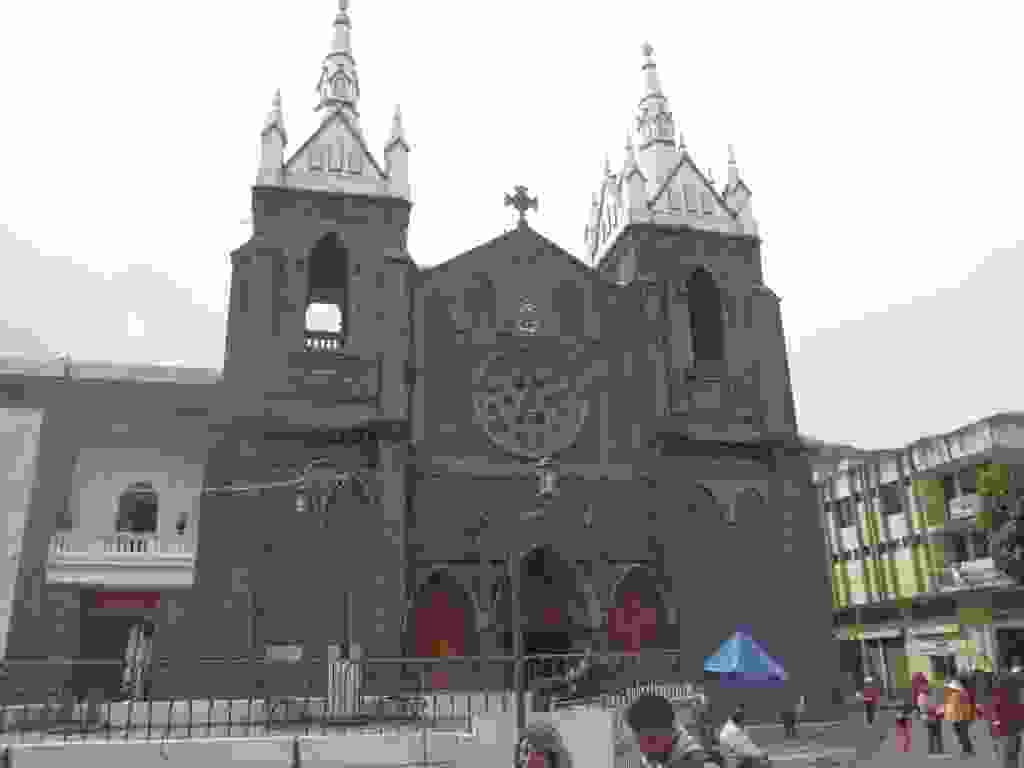
\includegraphics[width=\mywidth]{../wp-content/uploads/2015/06/P6204941-1024x768.jpg} \end{center}
\begin{center} 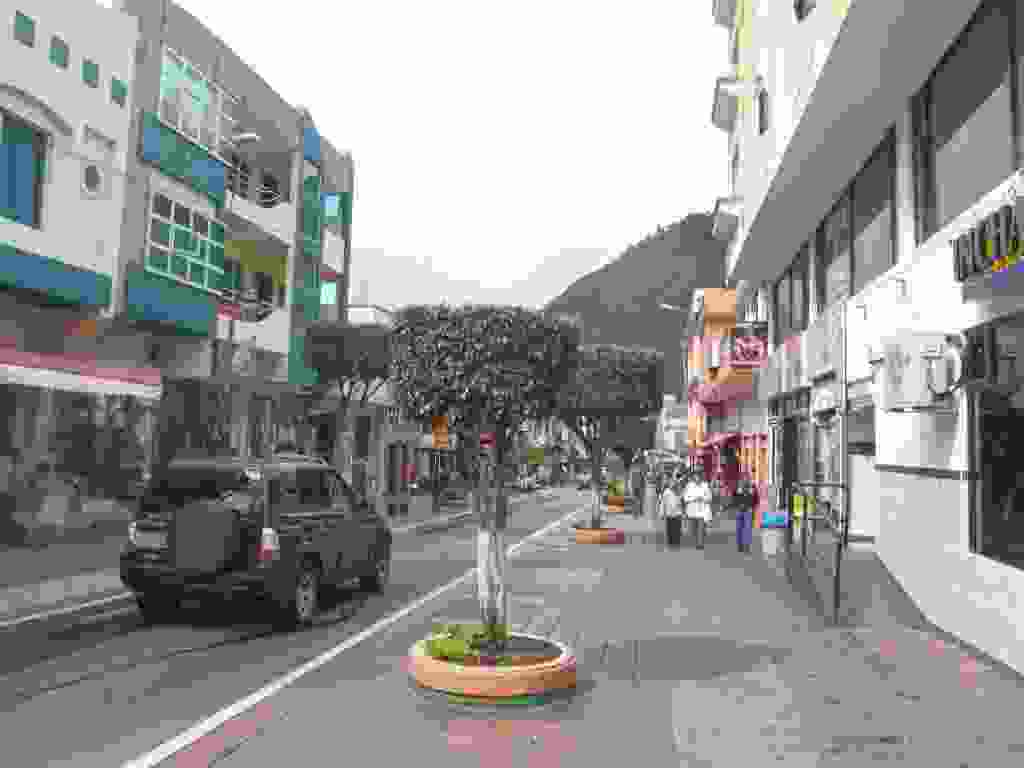
\includegraphics[width=\mywidth]{../wp-content/uploads/2015/06/P6204937-1024x768.jpg} \end{center}

Des stands vendent la canne à sucre sous toutes ses formes. 
\begin{center} 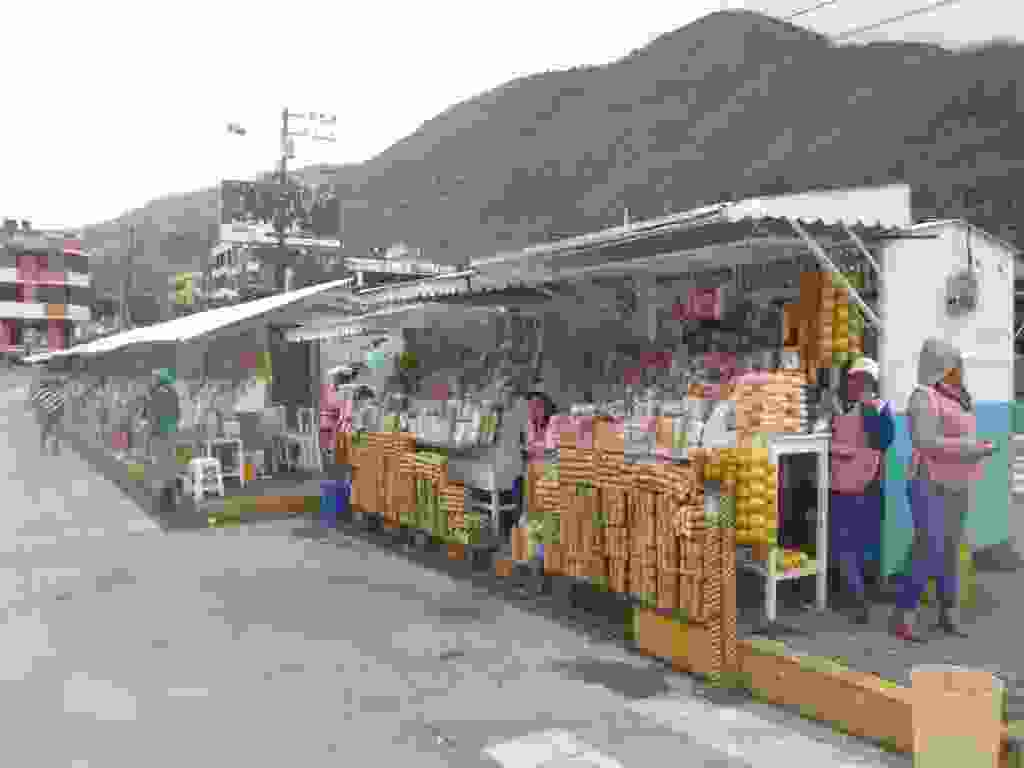
\includegraphics[width=\mywidth]{../wp-content/uploads/2015/06/P6214946-1024x768.jpg} \end{center}
\pagebreak

Au dessus de Baños, la Casa de l'Arbol avec parfois une belle vue. 
\begin{center} 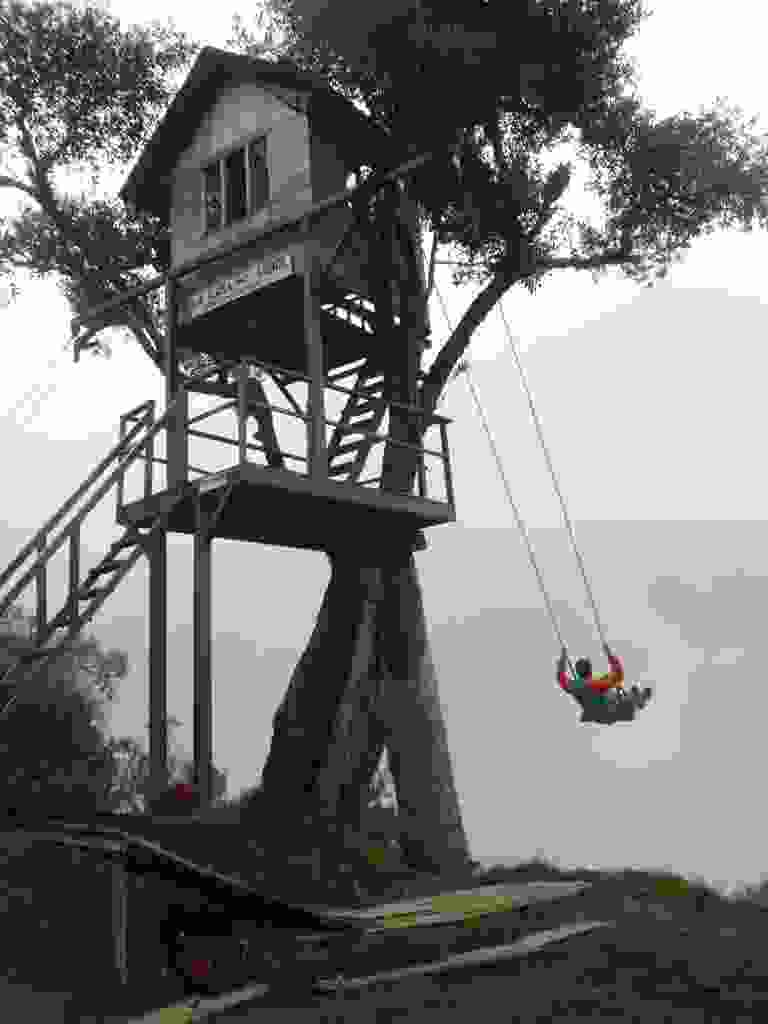
\includegraphics[height=\mywidth]{../wp-content/uploads/2015/06/P6214962-768x1024.jpg} \end{center}